\documentclass[12pt,a4paper]{article}
\usepackage[utf8]{inputenc}
\usepackage[T1]{fontenc}
\usepackage[margin=2.5cm]{geometry}
\usepackage{graphicx}
\usepackage{hyperref}
\usepackage{enumitem}
\usepackage{xcolor}
\usepackage{tikz}
\usetikzlibrary{shapes.geometric, arrows, positioning}
\usepackage{fancyhdr}
\usepackage{titlesec}
\usepackage{listings}

\definecolor{primary}{RGB}{220, 38, 38}
\definecolor{secondary}{RGB}{248, 113, 113}
\definecolor{codebg}{RGB}{248, 249, 250}

\lstset{
    backgroundcolor=\color{codebg},
    basicstyle=\ttfamily\small,
    breaklines=true,
    frame=single
}

\hypersetup{
    colorlinks=true,
    linkcolor=primary,
    urlcolor=primary
}

\pagestyle{fancy}
\fancyhf{}
\fancyhead[L]{Software Development Project}
\fancyhead[R]{System Design Document}
\fancyfoot[C]{\thepage}

\title{\textbf{System Design Document (SDD)}\\[0.5cm]\large Template}
\author{State University of Zanzibar (SUZA)}
\date{BSc Computer Science}

\begin{document}

\maketitle

\section*{Document Information}
\begin{tabular}{|l|l|}
\hline
\textbf{Project Name} & [Enter Project Name] \\
\hline
\textbf{Version} & 1.0 \\
\hline
\textbf{Date} & [Enter Date] \\
\hline
\textbf{Author(s)} & [Team Members] \\
\hline
\end{tabular}

\tableofcontents
\newpage

\section{Introduction}

\subsection{Purpose}
[Describe the purpose of this design document.]

\subsection{Scope}
[Define what aspects of the system this document covers.]

\subsection{Design Goals}
\begin{itemize}
    \item Scalability
    \item Maintainability
    \item Security
    \item Performance
    \item Usability
\end{itemize}

\section{System Architecture}

\subsection{Architecture Overview}
[Provide a high-level description of the system architecture.]

\subsection{Architecture Diagram}
[Insert or describe your system architecture diagram]

\begin{center}
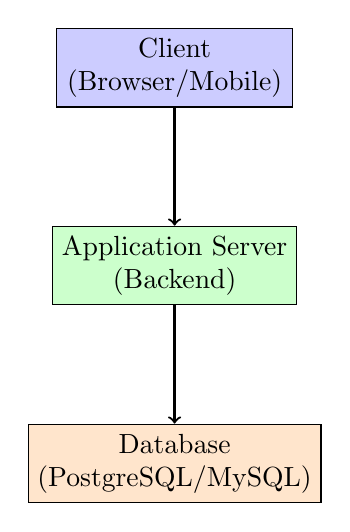
\begin{tikzpicture}[
    box/.style={rectangle, draw, minimum width=3cm, minimum height=1cm, align=center},
    arrow/.style={->, thick}
]
    % Example architecture
    \node[box, fill=blue!20] (client) {Client\\(Browser/Mobile)};
    \node[box, fill=green!20, below=1.5cm of client] (server) {Application Server\\(Backend)};
    \node[box, fill=orange!20, below=1.5cm of server] (db) {Database\\(PostgreSQL/MySQL)};

    \draw[arrow] (client) -- (server);
    \draw[arrow] (server) -- (db);
\end{tikzpicture}
\end{center}

\subsection{Architecture Pattern}
[Describe the architectural pattern used]
\begin{itemize}
    \item \textbf{Pattern:} [e.g., MVC, Microservices, Layered]
    \item \textbf{Justification:} [Why this pattern was chosen]
\end{itemize}

\section{Technology Stack}

\subsection{Frontend Technologies}
\begin{tabular}{|l|l|l|}
\hline
\textbf{Technology} & \textbf{Version} & \textbf{Purpose} \\
\hline
React / Vue / Angular & [version] & UI Framework \\
\hline
HTML5 & 5 & Markup \\
\hline
CSS3 / Tailwind & [version] & Styling \\
\hline
JavaScript / TypeScript & [version] & Client Logic \\
\hline
\end{tabular}

\subsection{Backend Technologies}
\begin{tabular}{|l|l|l|}
\hline
\textbf{Technology} & \textbf{Version} & \textbf{Purpose} \\
\hline
Node.js / Python / Java & [version] & Server Runtime \\
\hline
Express / Django / Spring & [version] & Web Framework \\
\hline
\end{tabular}

\subsection{Database}
\begin{tabular}{|l|l|l|}
\hline
\textbf{Technology} & \textbf{Type} & \textbf{Purpose} \\
\hline
PostgreSQL / MySQL & Relational & Primary Database \\
\hline
MongoDB & NoSQL & [if applicable] \\
\hline
Redis & In-Memory & Caching \\
\hline
\end{tabular}

\subsection{DevOps and Deployment}
\begin{tabular}{|l|l|}
\hline
\textbf{Tool} & \textbf{Purpose} \\
\hline
Git / GitHub & Version Control \\
\hline
Docker & Containerization \\
\hline
AWS / Heroku / Vercel & Hosting \\
\hline
\end{tabular}

\section{Database Design}

\subsection{Entity Relationship Diagram}
[Include or describe your ERD]

\subsection{Database Schema}

\textbf{Table: users}
\begin{tabular}{|l|l|l|l|}
\hline
\textbf{Column} & \textbf{Type} & \textbf{Constraints} & \textbf{Description} \\
\hline
id & INT & PRIMARY KEY, AUTO\_INCREMENT & User ID \\
\hline
username & VARCHAR(50) & UNIQUE, NOT NULL & Username \\
\hline
email & VARCHAR(100) & UNIQUE, NOT NULL & Email address \\
\hline
password\_hash & VARCHAR(255) & NOT NULL & Hashed password \\
\hline
created\_at & TIMESTAMP & DEFAULT NOW() & Creation date \\
\hline
\end{tabular}

\vspace{0.5cm}
\textbf{Table: [table\_name]}
[Repeat format for each table]

\subsection{Database Relationships}
\begin{itemize}
    \item users $\rightarrow$ orders (One-to-Many)
    \item orders $\rightarrow$ products (Many-to-Many)
    \item [Add more relationships]
\end{itemize}

\section{API Design}

\subsection{API Overview}
[Describe the API architecture - REST, GraphQL, etc.]

\subsection{API Endpoints}

\textbf{Authentication Endpoints}
\begin{tabular}{|l|l|l|l|}
\hline
\textbf{Method} & \textbf{Endpoint} & \textbf{Description} & \textbf{Auth} \\
\hline
POST & /api/auth/register & Register new user & No \\
\hline
POST & /api/auth/login & User login & No \\
\hline
POST & /api/auth/logout & User logout & Yes \\
\hline
\end{tabular}

\vspace{0.5cm}
\textbf{Resource Endpoints}
\begin{tabular}{|l|l|l|l|}
\hline
\textbf{Method} & \textbf{Endpoint} & \textbf{Description} & \textbf{Auth} \\
\hline
GET & /api/users & Get all users & Yes \\
\hline
GET & /api/users/:id & Get user by ID & Yes \\
\hline
PUT & /api/users/:id & Update user & Yes \\
\hline
DELETE & /api/users/:id & Delete user & Yes \\
\hline
\end{tabular}

\subsection{Request/Response Examples}

\textbf{POST /api/auth/register}

Request:
\begin{lstlisting}
{
    "username": "john_doe",
    "email": "john@example.com",
    "password": "securepassword123"
}
\end{lstlisting}

Response (Success - 201):
\begin{lstlisting}
{
    "success": true,
    "message": "User registered successfully",
    "data": {
        "id": 1,
        "username": "john_doe",
        "email": "john@example.com"
    }
}
\end{lstlisting}

\section{User Interface Design}

\subsection{UI/UX Principles}
\begin{itemize}
    \item Consistency across all pages
    \item Mobile-first responsive design
    \item Clear navigation and feedback
    \item Accessibility compliance
\end{itemize}

\subsection{Screen Layouts}
[Include wireframes or mockups for key screens]

\begin{enumerate}
    \item \textbf{Login Page:} [Description]
    \item \textbf{Dashboard:} [Description]
    \item \textbf{Main Feature Page:} [Description]
    \item \textbf{Settings:} [Description]
\end{enumerate}

\subsection{Navigation Flow}
[Describe how users navigate through the application]

\section{Security Design}

\subsection{Authentication}
\begin{itemize}
    \item Method: JWT / Session-based
    \item Token expiration: [time]
    \item Refresh token mechanism: [yes/no]
\end{itemize}

\subsection{Authorization}
\begin{itemize}
    \item Role-based access control (RBAC)
    \item User roles: Admin, User, Guest
\end{itemize}

\subsection{Data Protection}
\begin{itemize}
    \item Passwords hashed using bcrypt
    \item HTTPS for all communications
    \item Input validation and sanitization
    \item SQL injection prevention
    \item XSS protection
\end{itemize}

\section{Component Design}

\subsection{Component 1: [Component Name]}
\begin{itemize}
    \item \textbf{Purpose:} [What it does]
    \item \textbf{Responsibilities:} [List of responsibilities]
    \item \textbf{Dependencies:} [What it depends on]
    \item \textbf{Interface:} [How other components interact with it]
\end{itemize}

\section{Deployment Architecture}

\subsection{Deployment Diagram}
[Describe or include deployment diagram]

\subsection{Environment Configuration}
\begin{itemize}
    \item \textbf{Development:} localhost
    \item \textbf{Staging:} [staging URL]
    \item \textbf{Production:} [production URL]
\end{itemize}

\section{Appendices}

\subsection{Glossary}
[Technical terms and definitions]

\subsection{Revision History}
\begin{tabular}{|l|l|l|l|}
\hline
\textbf{Version} & \textbf{Date} & \textbf{Author} & \textbf{Changes} \\
\hline
1.0 & [date] & [name] & Initial version \\
\hline
\end{tabular}

\end{document}
